\subsection{Hasil Pengujian}
\subsubsection{Fashion-MNIST}
\begin{frame}{Hasil Pengujian terhadap Fashion-MNIST}
  \begin{center}
    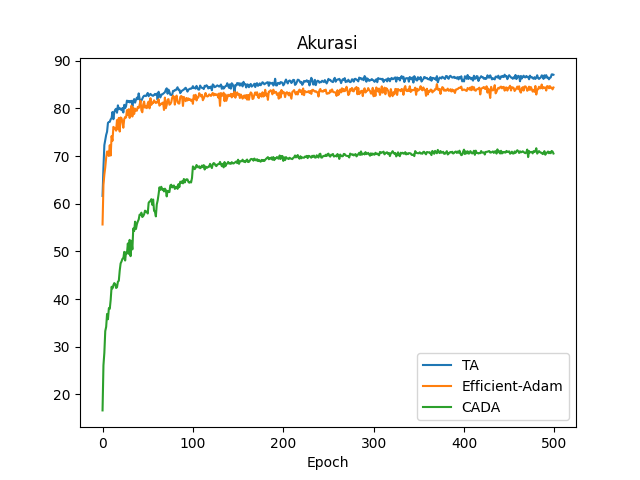
\includegraphics[width=6.5cm]{fashion_acc.png}
  \end{center}
  Akurasi tertinggi didapatkan oleh teknik gabungan, yang berada di sekitar 86\%. Sedangkan akurasi terendah didapatkan oleh CADA, di sekitar 70\%.
\end{frame}

\begin{frame}{Hasil Pengujian terhadap Fashion-MNIST}
  \begin{center}
    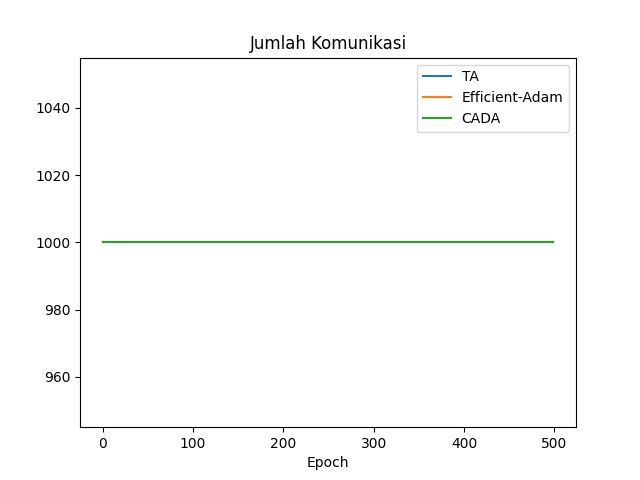
\includegraphics[width=6.5cm]{fashion_comms.png}
    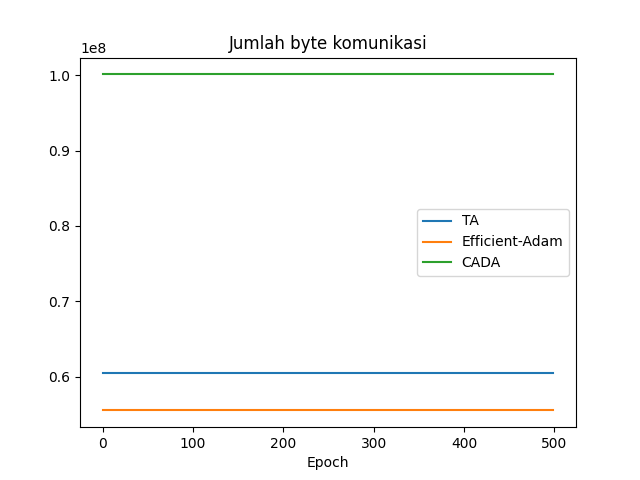
\includegraphics[width=6.5cm]{fashion_bits.png}
  \end{center}
  Jumlah komunikasi sama untuk setiap teknik, namun jumlah byte yang digunakan Efficient-Adam dan teknik gabungan jauh lebih sedikit dibandingkan CADA karena kompresi.
\end{frame}

\subsubsection{CIFAR10}
\begin{frame}{Hasil Pengujian terhadap CIFAR-10}
  \begin{center}
    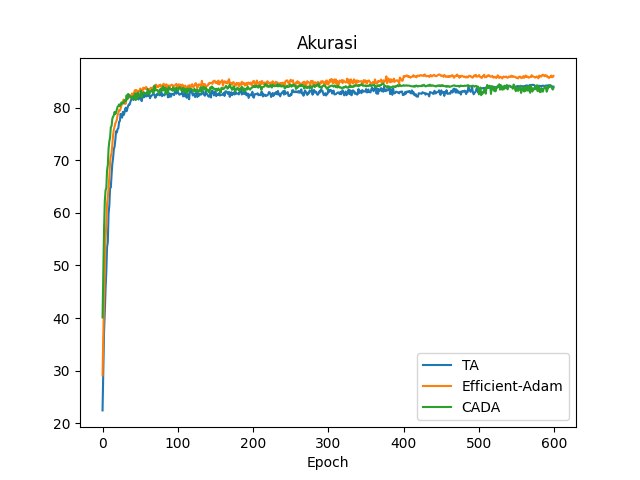
\includegraphics[width=6.5cm]{resnet_acc.png}
  \end{center}
  Akurasi yang didapatkan berada di sekitar 84-86\% untuk setiap teknik, dengan Efficient-Adam memiliki akurasi tertinggi.
\end{frame}

\begin{frame}{Hasil Pengujian terhadap CIFAR-10}
  \begin{center}
    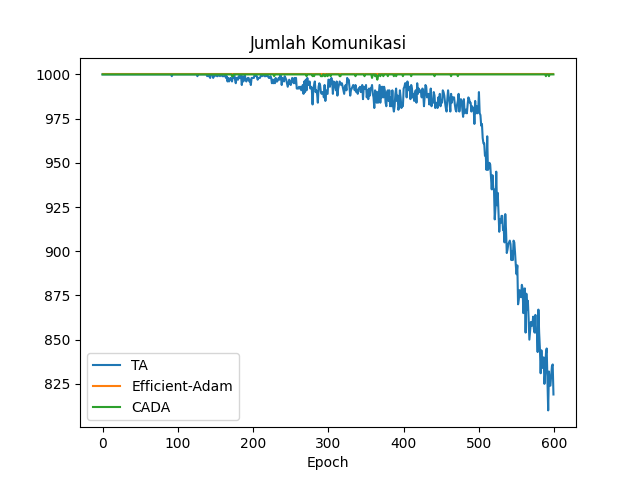
\includegraphics[width=6.5cm]{resnet_comms.png}
    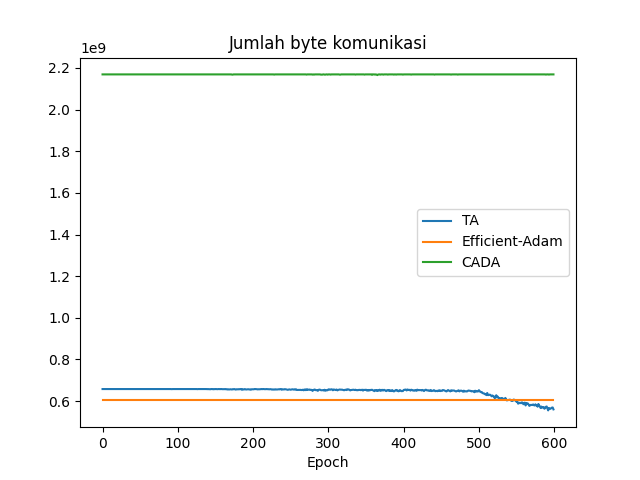
\includegraphics[width=6.5cm]{resnet_bits.png}
  \end{center}
  Jumlah komunikasi dikurangi paling banyak oleh teknik gabungan, dengan CADA mengurangi komunikasi pada beberapa epoch tertentu saja. Jumlah byte yang digunakan paling sedikit oleh Efficient-Adam, namun teknik gabungan mampu mengurangi jumlah byte karena jumlah komunikasi yang berkurang.
\end{frame}
